\section{Risultati}
Questa sezione è dedicata ai risultati sperimentali.
Nelle tabelle in seguito, con il termine \textit{slowfactor} ci riferiremo al rapporto fra il tempo di esecuzione, in secondi, di PDIP-LDL e QUADPROG.
In queste tabelle in grassetto sono evidenziati il massimo e minimo \textit{slowfactor}.


I files chiamati \texttt{ResultsEXP\{1,2,3\}.mat} contengono le strutture \texttt{MATLAB} che memorizzano i risultati dei sotto-esperimenti. Per il quarto sotto-esperimento sono state utilizzate le soluzioni già calcolate negli altri sotto-esperimenti.

Il numero nel nome del file indica il sotto-esperimento, ciascun file contiene tre strutture che raccolgono i risultati di ogni metodo nel seguente ordine: PDIP-LDL, PDIP-GMRES e QUADPROG.
La tabella \ref{tab:struct} descrive i campi della generica struttura.

\begin{table}[!h]
\centering
\begin{tabular}{r|l}
\textbf{experiment} & \textit{Stringa che identifica il sotto-esperimento.       }                                                                                                                                                                                      \\\hline
\textbf{method }    & \textit{Stringa che specifica quale dei tre metodi è stato utilizzato.                                                                                       }                                                                                     \\\hline
\textbf{times}      & \begin{tabular}[c]{@{}l@{}}\textit{Matrice di dimensione} $|parameters|\times nrepeat$ \\ \textit{che contiene i tempi di esecuzione del metodo per ogni}\\ \textit{valore }$\in$\textit{parameters e per ognuna delle }$nrepat$ \\ \textit{ripetizioni dell'esperimento}.\end{tabular}   \\\hline
\textbf{iterations} & \begin{tabular}[c]{@{}l@{}}\textit{Matrice di dimensione }$|parameters|\times nrepeat$ \\\textit{ che contiene il numero di iterazioni del metodo per ogni}\\ \textit{valore } $\in$ \textit{parameters e per ognuna delle }$nrepat$\\ \textit{ripetizioni dell'esperimento.}\end{tabular} \\\hline
\textbf{parameters} & \begin{tabular}[c]{@{}l@{}}\textit{Vettore che contiene i valori che verranno assunti dal parametro}\\ \textit{preso in esame nel sotto-esperimento corrente}.\end{tabular}                                                                               
\end{tabular}
\caption{Tabella che descrive i campi delle strutture che contengono i risultati sperimentali.}
\label{tab:struct}
\end{table}

\subsection{Scalabilità}

 In questo gruppo di esperimenti abbiamo voluto testare la scalabilità della nostra implementazione: fissando numero di vincoli $m$ e densità di $Q$, $\delta$, abbiamo fatto variare la \textit{dimensione dell'input} $n$. Analizziamo ora grafici e tabelle relative a tempi di esecuzione e numero di iterazioni. 

\begin{figure}[h!]
    \centering
    \begin{subfigure}[h]{0.5\textwidth}
        \centering
        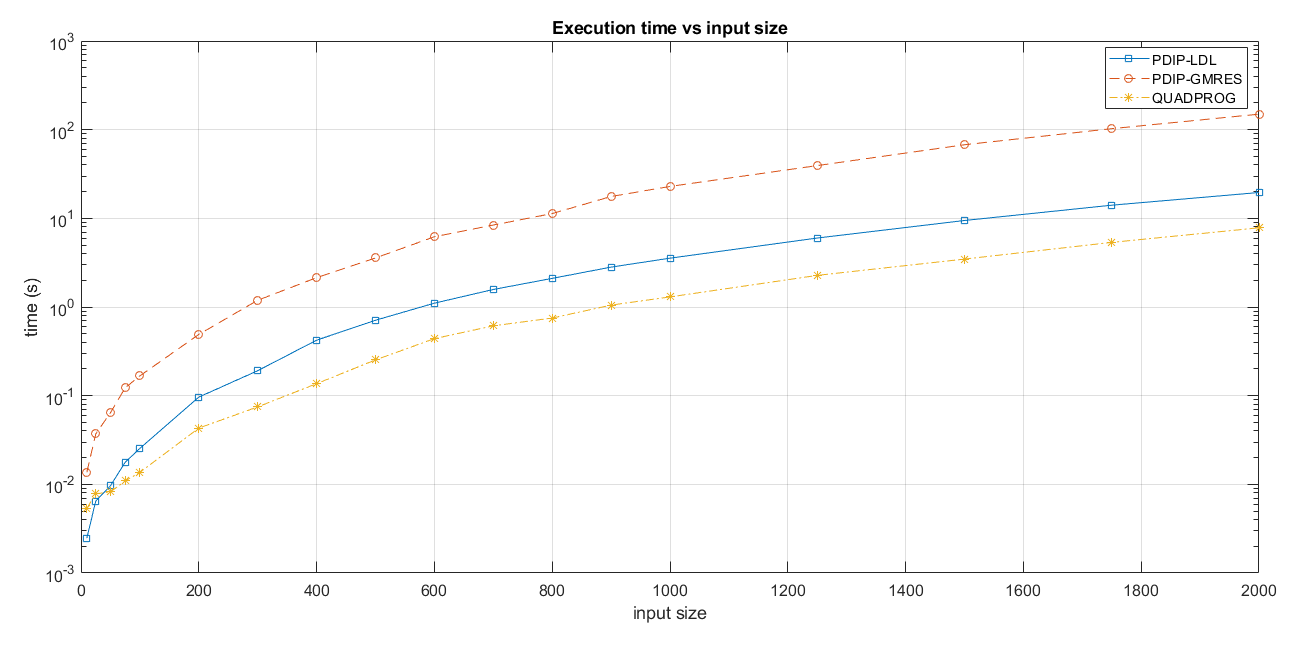
\includegraphics[height=4.52cm]{img/MU1.png}
    \caption{Confronto fra i tre metodi con asse delle y in \textit{log-scale}.\label{fig:exp111}}
    \end{subfigure}%
    ~ 
    \begin{subfigure}[h]{0.5\textwidth}
        \centering
                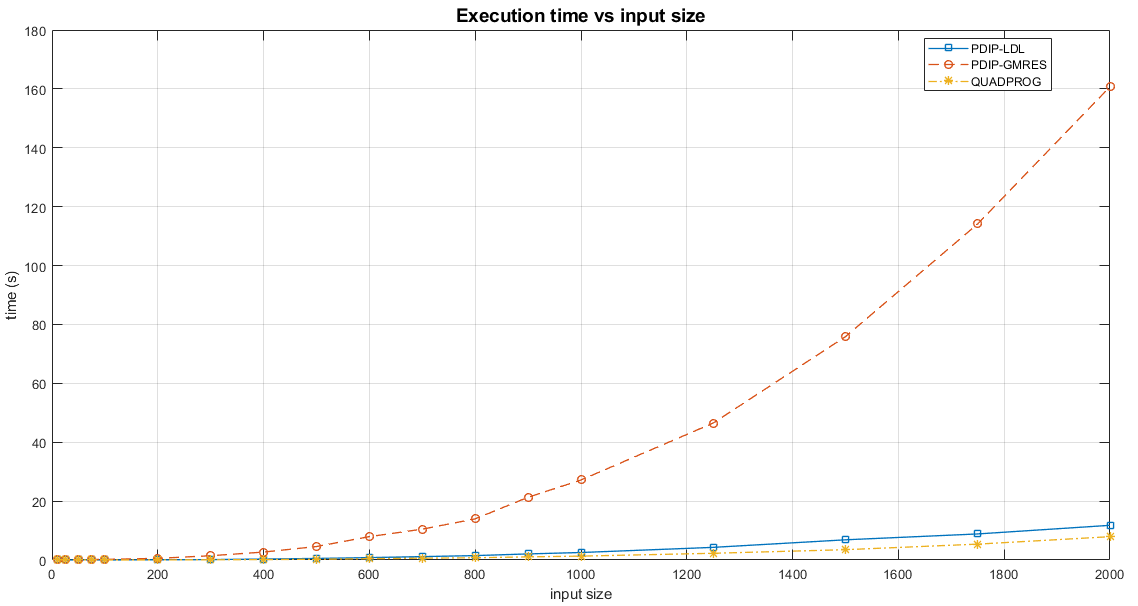
\includegraphics[height=4.4cm]{img/MU10.png}
    \caption{Confronto fra i tre metodi. \label{fig:exp112}}
    \end{subfigure}
    ~\newline
     \begin{subfigure}[h]{0.8\textwidth}
        \centering
                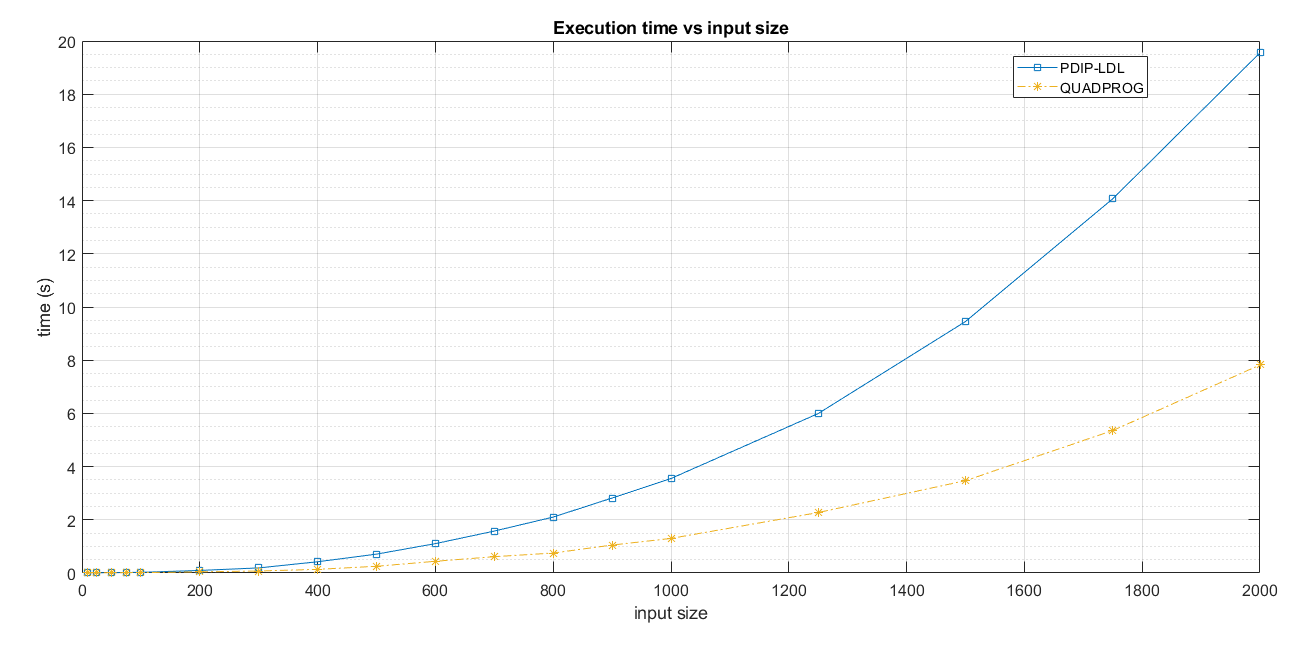
\includegraphics[height=6cm]{img/MU11.png}
    \caption{Grafico di confronto fra PIDP-LDL e QUADPROG. \label{fig:exp113}}
    \end{subfigure}
    \caption{Tempo di esecuzione, in secondi, all'aumentare della dimensione del problema $n$. \label{fig:exp1}}
\end{figure}



La Figura \ref{fig:exp1} ci permette di confrontare i tempi di completamento dei metodi analizzati; possiamo notare che l'andamento è esponenziale rispetto ad $n$ per tutti e tre i metodi.
In particolare:
\begin{itemize}
    \item in Fig.\ref{fig:exp112} la curva relativa al metodo PDIP-GMRES cresce con un esponente maggiore rispetto agli altri due metodi, questo a causa della presenza di metodo iterativo al suo interno, ossia GMRES, che all'aumentare di $n$ dovrà approssimare la soluzione di un sistema sempre più grande.
    
    \item confrontando i due metodi più veloci in Fig.\ref{fig:exp113} e Tab.\ref{tab:ldlqp2} possiamo notare come la nostra implementazione abbia scalabilità paragonabile a quella di QUADRPROG a meno di un fattore $\approx\times1.85$.

\end{itemize}

\begin{table}[!h]
\centering
\begin{tabular}{|l|c|c|c|c|c|c|c|c|}
\hline \textbf{input size}                  & \textbf{50}  & \textbf{75}  & \textbf{100} & \textbf{200}  & \textbf{300}  & \textbf{400}  & \textbf{500}  & \textbf{600}  \\\hline
\textbf{PDIP-LDL}                    & 0.0064       & 0.0177       & 0.0211       & 0.0575        & 0.1418        & 0.3251        & 0.5271        & 0.8170        \\
\textbf{QUADPROG}                    & 0.0069       & 0.0115       & 0.0137       & 0.0334        & 0.0737        & 0.1377        & 0.2590        & 0.4541        \\
\textbf{slowfactor} & \textbf{0.9259}       & 1.5432       & 1.5422       & 1.7229        & 1.9247        & \textbf{2.3617}        & 2.0351        & 1.7989        \\ \hline
\textbf{input size}                  & \textbf{700} & \textbf{800} & \textbf{900} & \textbf{1000} & \textbf{1250} & \textbf{1500} & \textbf{1750} & \textbf{2000} \\\hline
\textbf{PDIP-LDL}                    & 1.1532       & 1.4939       & 2.0655       & 2.5441        & 4.2911        & 6.8573        & 8.8513        & 11.7768       \\
\textbf{QUADPROG}                    & 0.6157       & 0.7584       & 1.0631       & 1.3172        & 2.2816        & 3.5041        & 5.3935        & 7.9170        \\
\textbf{\textit{slowfactor}} & 1.8728       & 1.9697       & 1.9428       & 1.9315        & 1.8808        & 1.9569        & 1.6411        & 1.4875  \\\hline     
\end{tabular}
    \caption{Tabelle contenenti la media dei tempi di esecuzione (s) di PDIP-LDL e QUADPROG relativi al primo sotto-esperimento. \label{tab:ldlqp2}}
    \end{table}
   
    
\begin{table}[!h]
\centering
\begin{tabular}{|l|c|c|c|c|c|c|c|c|}\hline
\textbf{input size} & \textbf{50}  & \textbf{75}  & \textbf{100} & \textbf{200}  & \textbf{300}  & \textbf{400}  & \textbf{500}  & \textbf{600}  \\\hline
\textbf{PDIP-LDL}   & 10.65\%      & 29.22\%      & 17.34\%      & 5.81\%        & 8.03\%        & 3.87\%        & 5.03\%        & 1.80\%        \\
\textbf{QUADPROG}   & 13.35\%      & 25.80\%      & 17.72\%      & 2.55\%        & 3.12\%        & 4.95\%        & 19.12\%       & 7.99\%        \\\hline
\textbf{input size} & \textbf{700} & \textbf{800} & \textbf{900} & \textbf{1000} & \textbf{1250} & \textbf{1500} & \textbf{1750} & \textbf{2000} \\\hline
\textbf{PDIP-LDL}   & 3.96\%       & 2.74\%       & 1.67\%       & 1.94\%        & 2.27\%        & 1.56\%        & 2.31\%        & 2.41\%        \\
\textbf{QUADPROG}   & 2.94\%       & 1.37\%       & 1.42\%       & 0.94\%        & 1.13\%        & 0.85\%        & 0.92\%        & 0.83\%     \\  \hline
\end{tabular}
    \caption{Tabella contenente la deviazione standard dei tempi di esecuzione di PDIP-LDL e QUADPROG relativi al primo sotto-esperimento. \label{tab:ldlqp1.1}}
\end{table}

La Tab. \ref{tab:ldlqp1.1} mostra come le prestazioni ottenute sono stabili anche in termini di deviazione standard; si nota un leggero aumento di quest'ultima sulle istanze piccole del problema in quanto una piccola variazione incide maggiormente sulla metrica.

La variazione dell'input-size non sembra invece influire in maniera significativa sul  numero di iterazioni necessarie alla convergenza dei metodi.
Il grafico in Fig.\ref{fig:exp1.2} mostra infatti come, a prescindere dal valore di $n$, PDIP impieghi circa 21 iterazioni mentre QUADPROG circa 7.

\begin{figure}[!h]
    \centering
    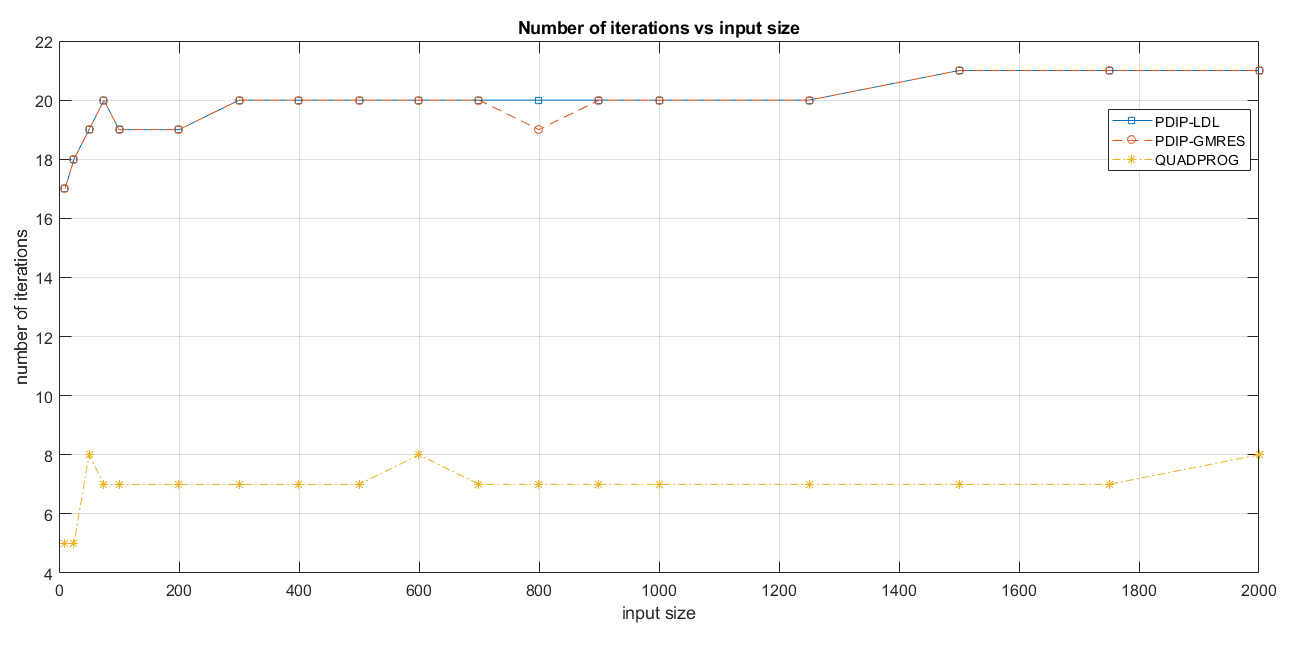
\includegraphics[width=\textwidth]{img/MU7.png}
    \caption{Il grafico mostra l'andamento del numero di iterazioni all'aumentare di $n$. \label{fig:exp1.2}}
\end{figure}

\subsection{Numero di Vincoli}

 In questo gruppo di esperimenti abbiamo voluto analizzare l'effetto che la variazione di $m$ ha sul tempo di convergenza dei metodi; $\delta$ ed $n$ rimangono fissati come in Tab. \ref{tab:param}.

\begin{figure}[h!]
    \centering
    \begin{subfigure}[h]{0.5\textwidth}
        \centering
        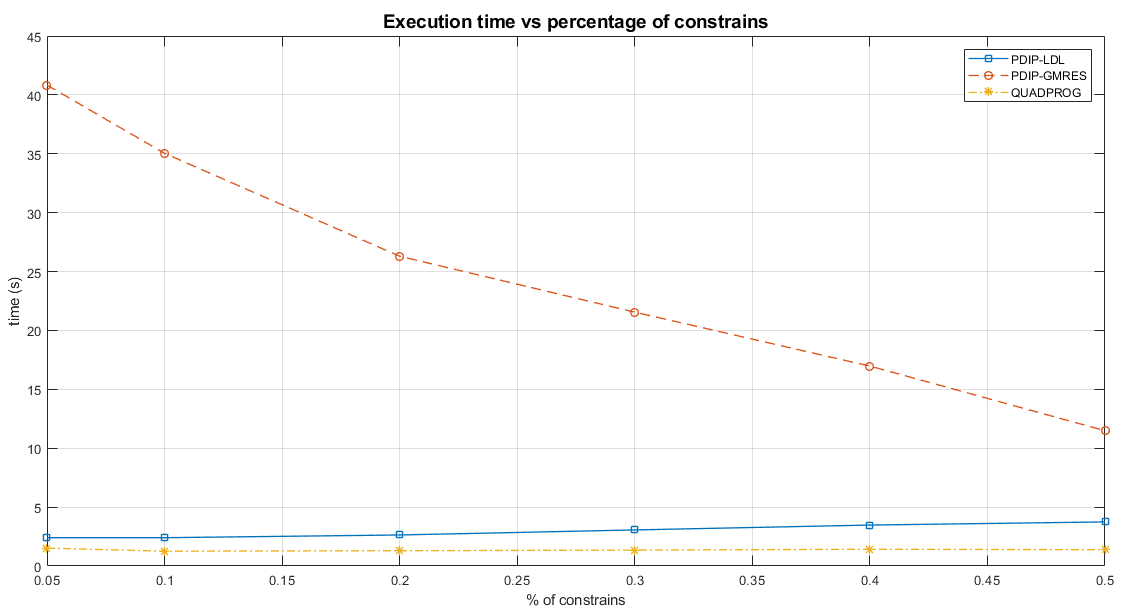
\includegraphics[width=\textwidth, height=2.42in]{img/MU2.png}
    \caption{Grafico di confronto fra i tempi di esecuzione dei tre metodi. \label{fig:exp2}}
    \end{subfigure}%
    ~ 
    \begin{subfigure}[h]{0.5\textwidth}
        \centering
         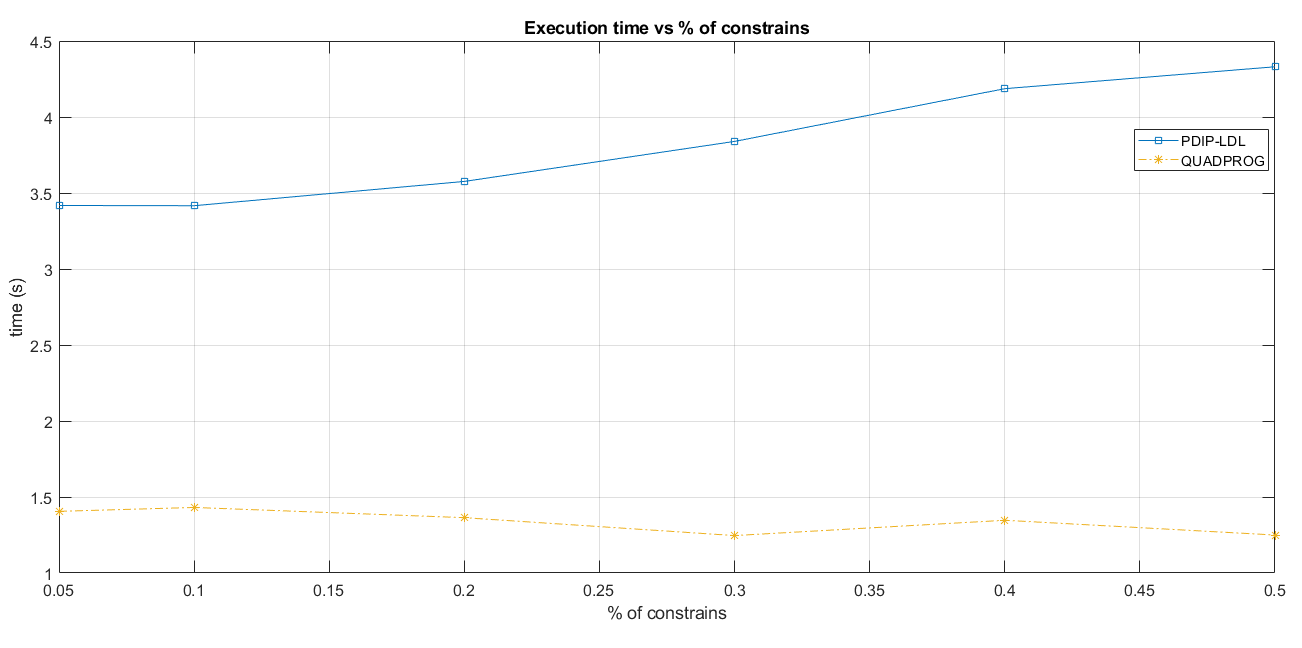
\includegraphics[width=\textwidth, height=2.4in]{img/MU3.png}
    \caption{Grafico di confronto fra PIDP-LDL e QUADPROG. \label{fig:exp2.1}}
    \end{subfigure}
    \caption{I grafici mostrano l'andamento del tempo di esecuzione, in secondi, all'aumentare del numero dei vincoli $m$; espresso in percentuale rispetto ad $n$. \label{fig:exp22}}
\end{figure}
 
in Fig.\ref{fig:exp2} GMRES impega meno tempo per covergere all'aumentare del numero di vincoli; questo perchè è più efficiente su matrici sparse: poichè il numero di elementi non-nulli in $A$ è sempre $n$, all'aumentare di $m$, la sparsità del sistema aumenta, confermando che le performance di GMRES su sistemi sparsi sono migliori.

Confrontando invece PDIP-LDL e QUADPROG in Fig.\ref{fig:exp2.1}, notiamo come l'aumentare del numero di vincoli impatti in modo negativo sulle performance della nostra implementazione, probabilmente a causa dell'aumento della dimensione del sistema da risolvere che penalizza l'approccio diretto. Anche il tempo di convergenza di QUADPROG aumenta con $m$, ma in modo meno netto. 

La Tabella \ref{tab:ldlqp2} conferma la stabilità del nostro metodo più veloce: si osservano infatti deviazioni standard trascurabili, dello stesso ordine di grandezza di QUADPROG; è possibile osservare anche che lo slowfactor aumenta in modo monotono al variare di $m$, rimanendo compreso nell'intervallo $[1.58, 2.7]$.

\begin{table}[!h]
\centering
\begin{tabular}{c|c|c|c|c|c|c}

$\mathbf{m}$            & \textbf{0.05} & \textbf{0.1} & \textbf{0.2} & \textbf{0.3} & \textbf{0.4} & \textbf{0.5} \\ \hline
\textbf{PDIP-LDL}                    & $2.401 \pm 2.6\%$       & $2.403 \pm 1.8\%$       & $2.634     \pm 2\%$   & $3.062 \pm 3\%$      & $3.476 \pm 1.9\%$      & $3.743 \pm 2.8\%$       \\
\textbf{QUADPROG}                    & $1.519 \pm 3.3\%$       & $1.256 \pm 2.4\%$       & $1.299 \pm 0.9\%$       & $1.351 \pm 1.6\%$       & $1.420 \pm 0.9\%$       & $1.382 \pm 3.6\%$       \\
\textbf{\textit{slowfactor}} &\textbf{1.581}        & 1.913       & 2.027       & 2.267       & 2.446       & \textbf{2.707} 
\end{tabular}
\caption{Tabella contenente media e deviazione standard dei tempi di esecuzione (s) di PDIP-LDL e QUADPROG relativi al secondo sotto-esperimento.\label{tab:ldlqp2}}
\end{table}

Infine, osserviamo che in Fig. \ref{fig:exp2.2} il numero di iterazioni diminuisce all'aumentare di $m$, questo però non vale per QUADPROG il cui numero di iterazioni non viene influenzato dalla frazione di vincoli rispetto alla dimensione dell'input.


\begin{figure}[!h]
    \centering
    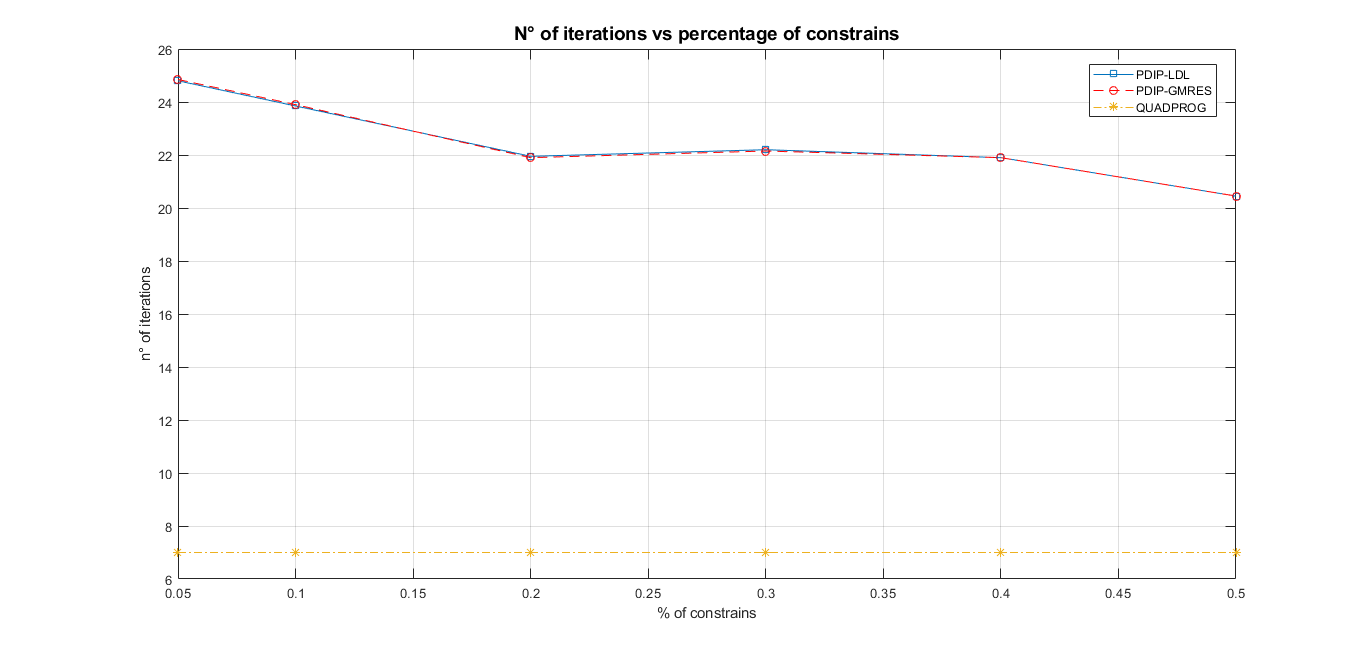
\includegraphics[width=\textwidth]{img/MU8.png}
    \caption{Numero di iterazioni all'aumentare di $m$. \label{fig:exp2.2}}
\end{figure}


\subsection{Densità}

 In questo gruppo di esperimenti abbiamo voluto testare qualora la densità della matrice $Q$ avesse effetti sui tempi di convergenza e il numero di iterazioni dei vari approcci coinvolti nella nostra analisi.

\begin{figure}[h]
    \centering
    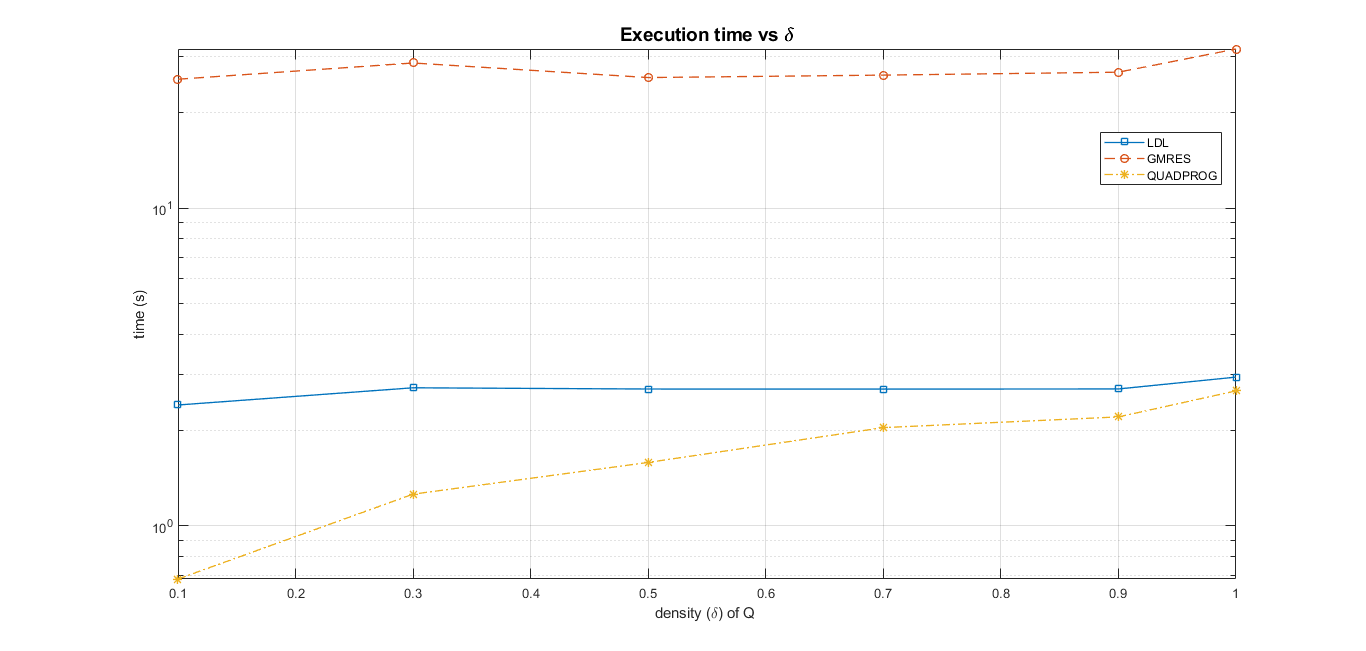
\includegraphics[width=\textwidth]{img/MU4.png}
    \caption{Tempo di esecuzione (in \textit{log-scale} sull'asse delle y) dei tre metodi all'aumentare della densità ($\delta$) di $Q$. \label{fig:exp3.1}}
\end{figure}
 
Da Fig. \ref{fig:exp3.1} si evince che l'aumento di $\delta$ ha un impatto critico sulle prestazioni di QUADPROG, mentre entrambe le versioni della nostra implementazione non sembrano risentire troppo dell'aumento di densità della matrice $Q$, con PDIP-LDL più veloce di un ordine di grandezza rispetto a PDIP-GMRES. 

 In Fig. \ref{fig:exp3.2}, il numero di iterazioni necessarie alla convergenza rimane stabile rispetto alla variazione di densità di $Q$ in tutti i metodi testati. 
 
 Confrontando infine i tempi di PDIP-LDL e QUADPROG in Tab. \ref{tab:ldlqp3}:
 \begin{itemize}
     \item il tempo di completamento della versione con risoluzione diretta della nostra implementazione rimane costante e stabile all'aumentare della densità
     \item il tempo di completamento di QUADPROG, invece, aumenta monotonamente
     \item di conseguenza lo slowfactor è massimo in corrispondenza del valore minimo di $\delta$, minimo viceversa; in generale la nostra implementazione è più lenta di un fattore $\approx \times1.8$.
 \end{itemize}
\begin{table}[!h]
\centering
\begin{tabular}{l|c|c|c|c|c|c}
\textbf{density}                     & \textbf{0.1} & \textbf{0.3} & \textbf{0.5} & \textbf{0.7} & \textbf{0.9} & \textbf{1.0} \\ \hline
\textbf{PDIP-LDL}                    & $2.401 \pm 1.2\%$       & $2.719 \pm 2.8\%$       & $2.695  \pm 2\%$       & $2.694 \pm 2.2\%$       & $2.696 \pm 2.3\%$       & $2.938  \pm 2.4\%$       \\
\textbf{QUADPROG}                    & $0.681  \pm 2.2\%$      & $1.258  \pm 5\%$       & $1.583 \pm 2.8\%$       & $2.038 \pm 1.5\%$       & $2.202 \pm 1.1\%$       & $2.659 \pm 5.9\%$       \\
\textbf{\textit{slowfactor}} & \textbf{3.526}       & 2.161       & 1.701       & 1.321       & 1.224       & \textbf{1.104}
\end{tabular}
\caption{Tabella contenente media e deviazione standard dei tempi di esecuzione (s) di PDIP-LDL e QUADPROG relativi al terzo sotto-esperimento. \label{tab:ldlqp3}}
\end{table}


\begin{figure}[!h]
    \centering
    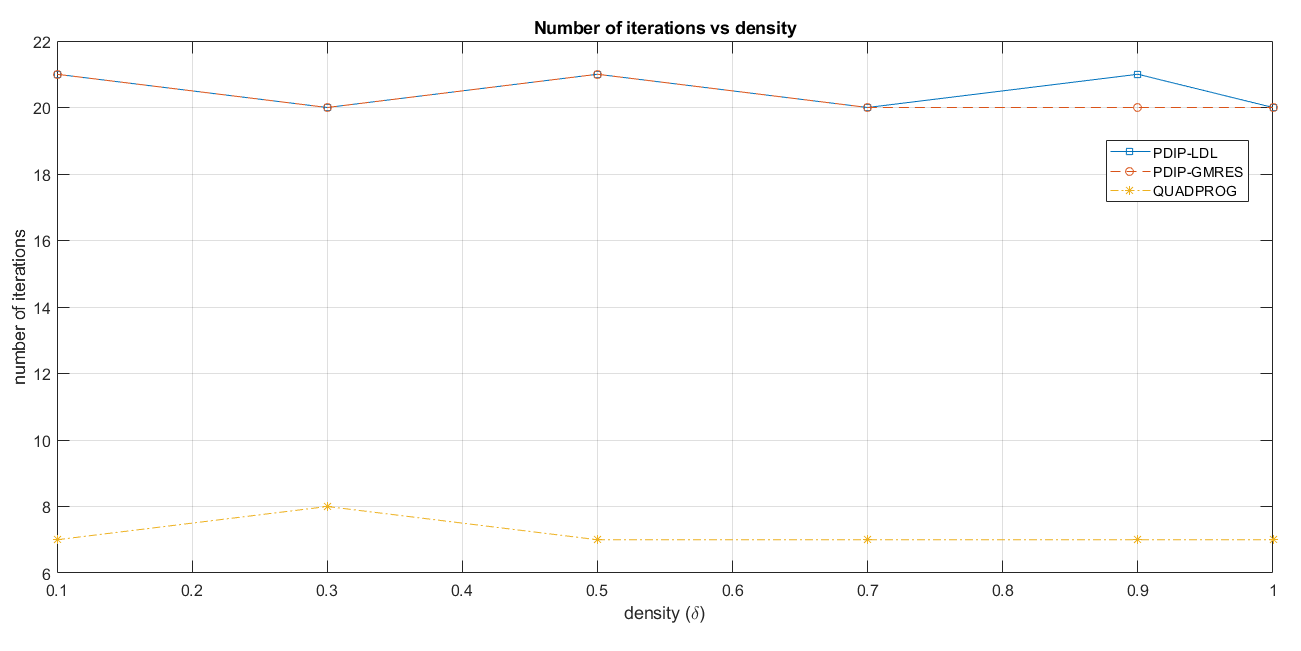
\includegraphics[width=\textwidth, height = 6.7cm]{img/MU9.png}
    \caption{Grafico dell'andamento del numero di iterazioni all'aumentare di $\delta$. \label{fig:exp3.2}}
\end{figure}

\subsection{Convergenza e Accuratezza della Soluzione}

Per i risultati in questa sezione sono state effettuate 20 esecuzioni fissando il problema come in Tab. \ref{tab:param}.
Per analizzare la convergenza dell'implementazione proposta, abbiamo collezionato i complementary gap ad ogni iterazione di PDIP sia in versione GMRES, che LDL.

Il grafico in Fig. \ref{fig:gap} mostra come varia - in scala logaritmica sull'asse delle y - ad ogni iterazione la media dei complementary gap: in entrambe le varianti della nostra implementazione il gap decresce monotonamente ad ogni iterazione successiva alla seconda e le prestazioni sono in linea con quelle attese.

\begin{figure}[!h]
    \centering
    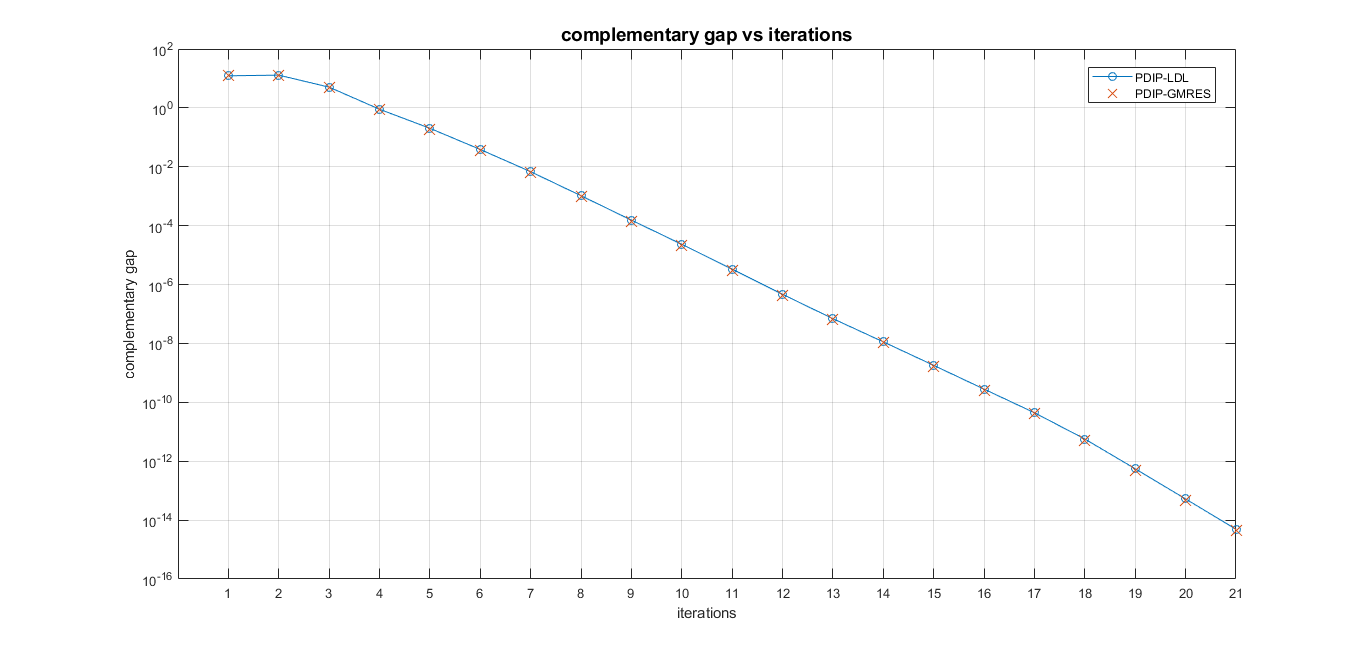
\includegraphics[width=\textwidth, height = 7.5cm]{img/MU6.png}
    \caption{Andamento del gap (in \textit{log-scale} sull'asse delle y) all'aumentare delle iterazioni. \label{fig:gap}}
\end{figure}

La seconda parte di questo esperimento ha l'obiettivo di valutare l'accuratezza della soluzione $(x, \lambda_{eq}, \lambda_s)$ dal nostro metodo. A questo proposito confrontiamo i residui finali e le triple restituite da PDIP-GMRES e PDIP-LDL fra di loro e con quella di QUADPROG. 

Come metrica di confronto per le triple abbiamo scelto di usare la norma della differenza fra i vettori soluzione $\norm{\delta_v}$ :

\begin{equation}\label{ep:acc}
     \norm{v_{M1} - v_{M2}} \;\;\;\;\;\;\;\;\; \mathrm{con} \;\;\; v\in \{ x, \lambda_{eq}, \lambda_s\} \;\; \mathrm{e} \;\; M_i \in \{{\scriptsize\mathit{PDIP-LDL},\; \mathit{PDIP-GMRES}, \; \mathit{QUADPROG}}\}
\end{equation}

In Tab. \ref{tab:normx} e \ref{tab:norml} sono riportate medie e deviazioni standard - su 20 esecuzioni - delle metriche, calcolate come in \ref{ep:acc}, rispettivamente per i vettori $x$ e $\lambda$.   

\begin{table}[!h]
\centering
\begin{tabular}{c|c|l|c}
$\mathbf{\norm{\delta x}}$ & \multicolumn{2}{c|}{\textbf{PDIP-GMRES}}         & \textbf{QUADPROG}          \\ \hline
\textbf{PDIP-LDL}            & \multicolumn{2}{c|}{$3.3856\cdot10^{-13}\pm6\%$} & $4.3127\cdot10^{-3}\pm0\%$ \\ \hline
\textbf{PDIP-GMRES}          & \multicolumn{2}{c|}{}                            & $4.3127\cdot10^{-3}\pm0\%$
\end{tabular}
\caption{Media e deviazione standard, sulle 20 ripetizioni, della norma della differenza fra i vettori soluzione.\label{tab:normx}}
\end{table}

\begin{table}[!h]
\begin{tabular}{c|c|c|c|c|}
      $\mathbf{\norm{\delta\lambda}}$             & \multicolumn{2}{c|}{\textbf{PDIP-LDL}}                                        & \multicolumn{2}{c|}{\textbf{PDIP-GMRES}}                                      \\ \hline
\textbf{PDIP-GMRES} & $1.6224\cdot10^{-13}\pm11\%$          & $1.1201\cdot10^{-12}\pm5.4\%$         & \multicolumn{2}{c|}{ }                                                        \\ 
\textbf{QUADPROG}   & $1.5712\cdot10^{-3}\pm0\%$            & $5.3517\cdot10^{-3}\pm0\%$            & $1.5712\cdot10^{-3}\pm0\%$            & $5.3517\cdot10^{{-3}}\pm0\%$          \\
                    & $\norm{ \delta\lambda_{eqlin} }$ & $\norm{ \delta\lambda_{s} }$ & $\norm{ \delta\lambda_{eqlin} }$ & $\norm{ \delta\lambda_{s} }$
\end{tabular}
\caption{Media e deviazione standard, sulle 20 ripetizioni, della norma della differenza fra i moltiplicatori lagrangiani soluzione dei metodi testati.\label{tab:norml}}
\end{table}

\begin{table}[!h]
\centering
\begin{tabular}{c|c|c}
\textbf{}           & $\mathbf{\norm{r_p}}$ & $\mathbf{\norm{r_d}}$ \\\hline
\textbf{PDIP-LDL} &      $1.1741\cdot10^{-15} \pm8.9\%$                 &           $1.3726\cdot10^{-14} \pm11.4\%$             \\\hline
\textbf{PDIP-GMRES}   &        $9.0965\cdot10^{-14} \pm13.3\%$               &            $1.1016\cdot10^{-12} \pm5.3\%$           \\\hline
\textbf{QUADPROG}   &      $9.8679\cdot10^{-16} \pm0\%$                &            $9.3234\cdot10^{-15} \pm0.1\%$   \\    
\end{tabular}
\caption{Tabella che riporta la media e deviazione standard su 20 esecuzioni della norma dei residui primali e duali finali dei tre metodi in analisi.}
\label{tab:res}
\end{table}

Le soluzioni ottenute dall'esecuzione diretta e iterativa di PDIP risultano pressocchè identiche: sia $\norm{\delta x}$ che $\norm{\delta\lambda}$ sono dell'ordine di $10^{-13}$; ed entrambe queste soluzioni sono uguali a quella trovata da QUADPROG a meno di un fattore di $10^{-3}$.

La Tabella \ref{tab:res} conferma ulteriormente la precisione della nostra implementazione: 
\begin{itemize}
    \item l'accuratezza raggiunta è paragonabile a quella di QUADPROG infatti sia il residuo primale, che duale sono maggiori di circa un ordine di grandezza rispetto alla built-in di \texttt{MATLAB}; probabilmente il nostro metodo potrebbe raggiungere precisione dello stesso ordine di grandezza di QUADPROG scegliendo una soglia $\eps$ più bassa rispetto a quella usata nei nostri esperimenti ($10^{-14}$), impiegando però più iterazioni e risultando più lento
    \item durante tutta la fase sperimentale abbiamo osservato deviazioni standard più alte per la nostra implementazione. Questo fenomeno può essere spiegato dalla presenza di una parte randomica nel nostro metodo, precisamente in \ref{eq:startl} durante la generazione della tripla iniziale: $\lambda_{eq}$ viene inizializzato con reali casuali, influenzando anche l'inizializzazione di $\lambda_s$; QUADPROG invece inizializza sempre $(x^0, \lambda_{eq}^0, \lambda_s^0) = 1$, con risultati finali di conseguenza più simili fra loro.
\end{itemize}

Concludendo la nostra implementazione, sia in versione diretta, che iterativa, può essere quindi considerata stabile e accurata rispetto alla built-in di \texttt{MATLAB} sia in termini di tempi ed iterazioni di convergenza, che di precisione del risultato finale.